%!TEX root=../Thesis.tex
\begin{figure}[ht]
\centering
\begin{subfigure}[b]{0.45\textwidth}
    \centering
    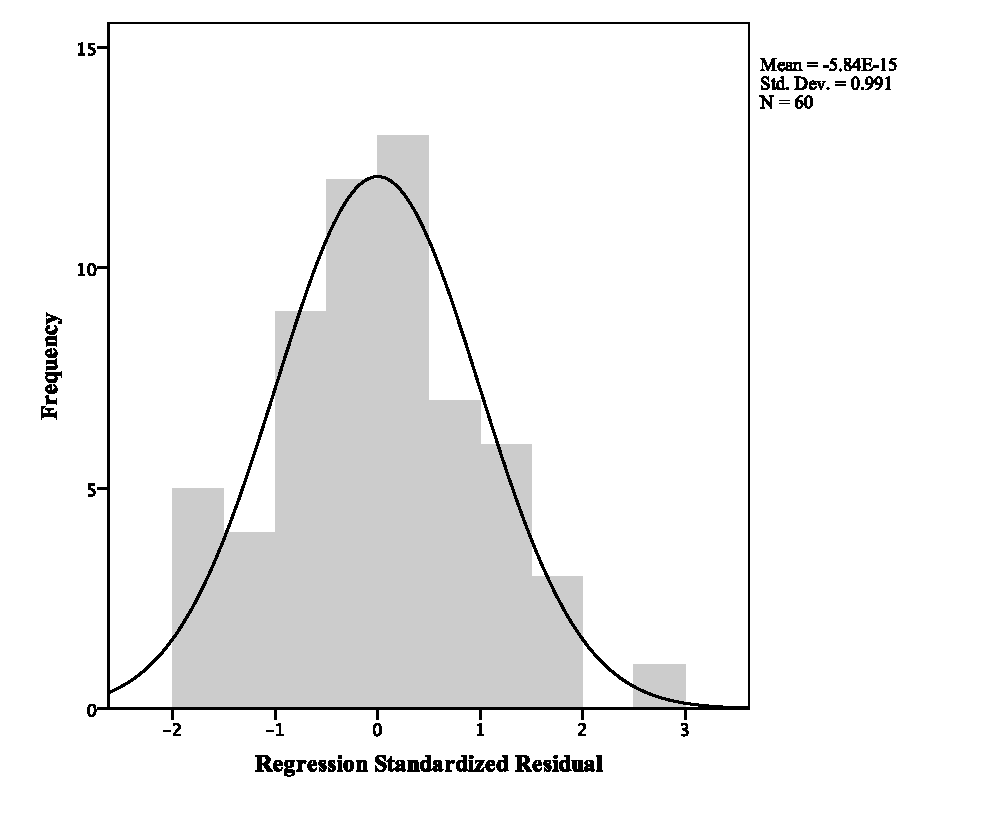
\includegraphics[width=\textwidth]{images/secondary/max/MaxHistogram.eps}
    \caption{Histogram}
    \label{fig:sec_max_hist}
\end{subfigure}
\quad
\begin{subfigure}[b]{0.45\textwidth}
    \centering
    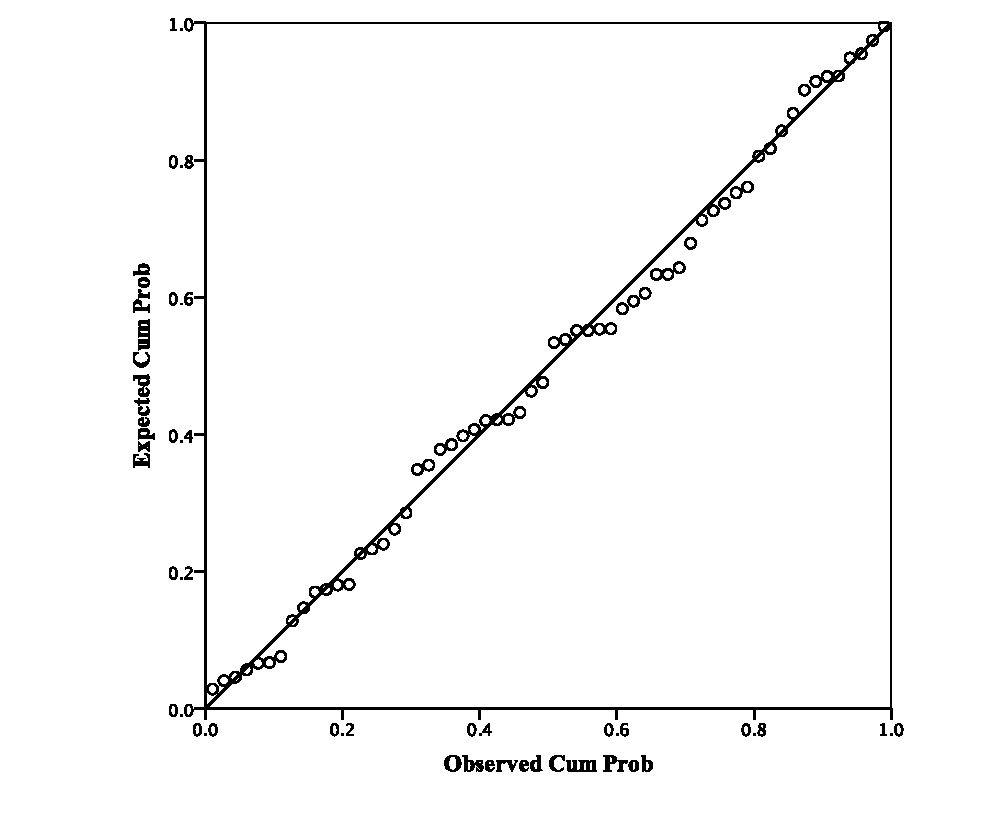
\includegraphics[width=\textwidth]{images/secondary/max/MaxP-P.eps}
    \caption{P-P plot}
    \label{fig:sec_max_PP}
\end{subfigure}
\caption{Normality graphs for max. tap pressure and duration. The histogram shows an approximate normal distribution. The P-P plot shows little deviation from the origin line, further proving a normal distribution of samples.}
\end{figure}
\par\bigskip
\par\bigskip
\begin{figure}[ht]
\begin{subfigure}[b]{0.45\textwidth}
    \centering
    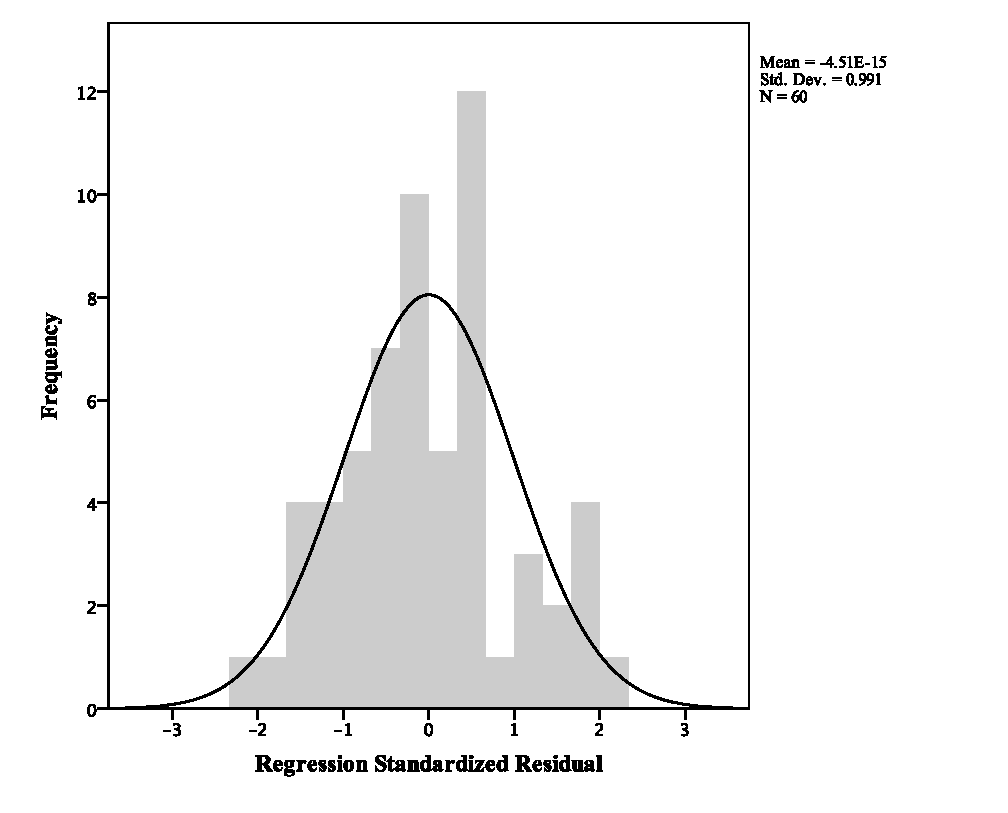
\includegraphics[width=\textwidth]{images/secondary/avg/AvgHistogram.eps}
    \caption{Histogram}
    \label{fig:sec_avg_hist}
\end{subfigure}
\quad
\begin{subfigure}[b]{0.45\textwidth}
    \centering
    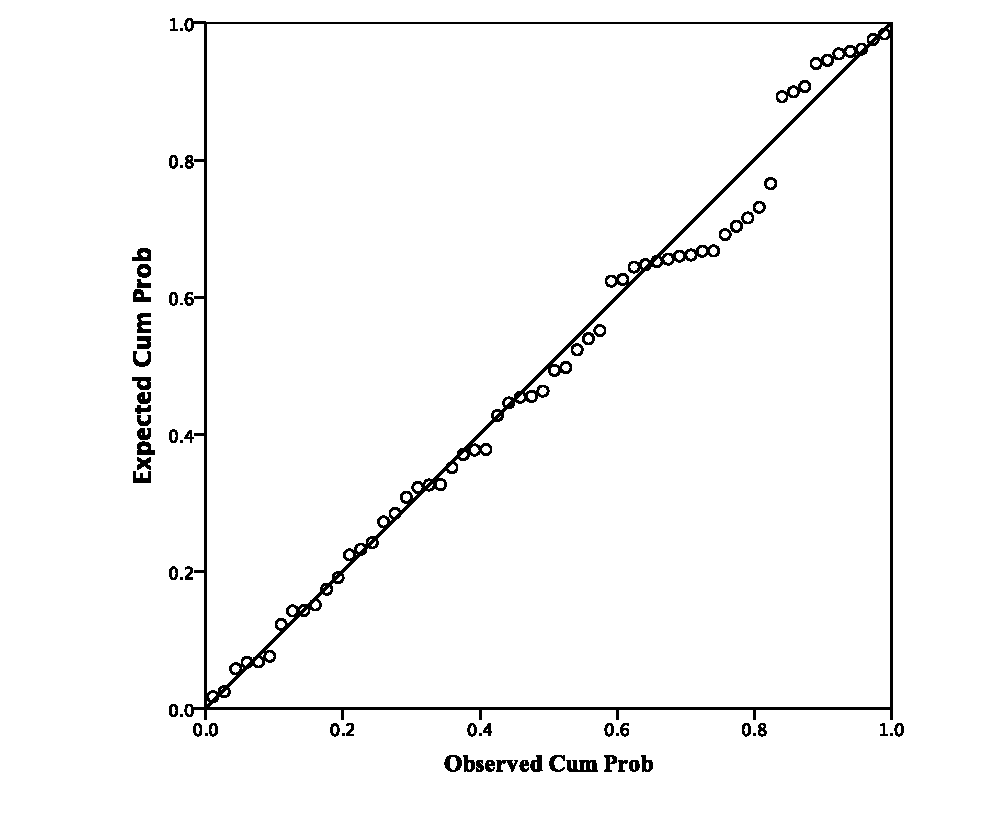
\includegraphics[width=\textwidth]{images/secondary/avg/AvgP-P.eps}
    \caption{P-P plot}
    \label{fig:sec_avg_PP}
\end{subfigure}
\caption{Normality graphs for avg. tap pressure and duration. The histogram shows an approximate normal distribution. The P-P plot shows little deviation from the origin line except at the top right, where it deviates a little more. Still, the deviation is not large enough to warrant any concerns over normal distribution of samples.}
\end{figure}